
%% bare_jrnl.tex
%% V1.3
%% 2007/01/11
%% by Michael Shell
%% see http://www.michaelshell.org/
%% for current contact information.
%%
%% This is a skeleton file demonstrating the use of IEEEtran.cls
%% (requires IEEEtran.cls version 1.7 or later) with an IEEE journal paper.
%%
%% Support sites:
%% http://www.michaelshell.org/tex/ieeetran/
%% http://www.ctan.org/tex-archive/macros/latex/contrib/IEEEtran/
%% and
%% http://www.ieee.org/



% *** Authors should verify (and, if needed, correct) their LaTeX system  ***
% *** with the testflow diagnostic prior to trusting their LaTeX platform ***
% *** with production work. IEEE's font choices can trigger bugs that do  ***
% *** not appear when using other class files.                            ***
% The testflow support page is at:
% http://www.michaelshell.org/tex/testflow/


%%*************************************************************************
%% Legal Notice:
%% This code is offered as-is without any warranty either expressed or
%% implied; without even the implied warranty of MERCHANTABILITY or
%% FITNESS FOR A PARTICULAR PURPOSE! 
%% User assumes all risk.
%% In no event shall IEEE or any contributor to this code be liable for
%% any damages or losses, including, but not limited to, incidental,
%% consequential, or any other damages, resulting from the use or misuse
%% of any information contained here.
%%
%% All comments are the opinions of their respective authors and are not
%% necessarily endorsed by the IEEE.
%%
%% This work is distributed under the LaTeX Project Public License (LPPL)
%% ( http://www.latex-project.org/ ) version 1.3, and may be freely used,
%% distributed and modified. A copy of the LPPL, version 1.3, is included
%% in the base LaTeX documentation of all distributions of LaTeX released
%% 2003/12/01 or later.
%% Retain all contribution notices and credits.
%% ** Modified files should be clearly indicated as such, including  **
%% ** renaming them and changing author support contact information. **
%%
%% File list of work: IEEEtran.cls, IEEEtran_HOWTO.pdf, bare_adv.tex,
%%                    bare_conf.tex, bare_jrnl.tex, bare_jrnl_compsoc.tex
%%*************************************************************************

% Note that the a4paper option is mainly intended so that authors in
% countries using A4 can easily print to A4 and see how their papers will
% look in print - the typesetting of the document will not typically be
% affected with changes in paper size (but the bottom and side margins will).
% Use the testflow package mentioned above to verify correct handling of
% both paper sizes by the user's LaTeX system.
%
% Also note that the "draftcls" or "draftclsnofoot", not "draft", option
% should be used if it is desired that the figures are to be displayed in
% draft mode.
%
\documentclass[journal]{IEEEtran}
\usepackage{blindtext}
\usepackage{graphicx}

% Some very useful LaTeX packages include:
% (uncomment the ones you want to load)


% *** MISC UTILITY PACKAGES ***
%
%\usepackage{ifpdf}
% Heiko Oberdiek's ifpdf.sty is very useful if you need conditional
% compilation based on whether the output is pdf or dvi.
% usage:
% \ifpdf
%   % pdf code
% \else
%   % dvi code
% \fi
% The latest version of ifpdf.sty can be obtained from:
% http://www.ctan.org/tex-archive/macros/latex/contrib/oberdiek/
% Also, note that IEEEtran.cls V1.7 and later provides a builtin
% \ifCLASSINFOpdf conditional that works the same way.
% When switching from latex to pdflatex and vice-versa, the compiler may
% have to be run twice to clear warning/error messages.



% *** CITATION PACKAGES ***
%
%\usepackage{cite}
% cite.sty was written by Donald Arseneau
% V1.6 and later of IEEEtran pre-defines the format of the cite.sty package
% \cite{} output to follow that of IEEE. Loading the cite package will
% result in citation numbers being automatically sorted and properly
% "compressed/ranged". e.g., [1], [9], [2], [7], [5], [6] without using
% cite.sty will become [1], [2], [5]--[7], [9] using cite.sty. cite.sty's
% \cite will automatically add leading space, if needed. Use cite.sty's
% noadjust option (cite.sty V3.8 and later) if you want to turn this off.
% cite.sty is already installed on most LaTeX systems. Be sure and use
% version 4.0 (2003-05-27) and later if using hyperref.sty. cite.sty does
% not currently provide for hyperlinked citations.
% The latest version can be obtained at:
% http://www.ctan.org/tex-archive/macros/latex/contrib/cite/
% The documentation is contained in the cite.sty file itself.






% *** GRAPHICS RELATED PACKAGES ***
%
\ifCLASSINFOpdf
  % \usepackage[pdftex]{graphicx}
  % declare the path(s) where your graphic files are
  % \graphicspath{{../pdf/}{../jpeg/}}
  % and their extensions so you won't have to specify these with
  % every instance of \includegraphics
  % \DeclareGraphicsExtensions{.pdf,.jpeg,.png}
\else
  % or other class option (dvipsone, dvipdf, if not using dvips). graphicx
  % will default to the driver specified in the system graphics.cfg if no
  % driver is specified.
  % \usepackage[dvips]{graphicx}
  % declare the path(s) where your graphic files are
  % \graphicspath{{../eps/}}
  % and their extensions so you won't have to specify these with
  % every instance of \includegraphics
  % \DeclareGraphicsExtensions{.eps}
\fi
% graphicx was written by David Carlisle and Sebastian Rahtz. It is
% required if you want graphics, photos, etc. graphicx.sty is already
% installed on most LaTeX systems. The latest version and documentation can
% be obtained at: 
% http://www.ctan.org/tex-archive/macros/latex/required/graphics/
% Another good source of documentation is "Using Imported Graphics in
% LaTeX2e" by Keith Reckdahl which can be found as epslatex.ps or
% epslatex.pdf at: http://www.ctan.org/tex-archive/info/
%
% latex, and pdflatex in dvi mode, support graphics in encapsulated
% postscript (.eps) format. pdflatex in pdf mode supports graphics
% in .pdf, .jpeg, .png and .mps (metapost) formats. Users should ensure
% that all non-photo figures use a vector format (.eps, .pdf, .mps) and
% not a bitmapped formats (.jpeg, .png). IEEE frowns on bitmapped formats
% which can result in "jaggedy"/blurry rendering of lines and letters as
% well as large increases in file sizes.
%
% You can find documentation about the pdfTeX application at:
% http://www.tug.org/applications/pdftex





% *** MATH PACKAGES ***
%
\usepackage[cmex10]{amsmath}
\usepackage{amsfonts}
% A popular package from the American Mathematical Society that provides
% many useful and powerful commands for dealing with mathematics. If using
% it, be sure to load this package with the cmex10 option to ensure that
% only type 1 fonts will utilized at all point sizes. Without this option,
% it is possible that some math symbols, particularly those within
% footnotes, will be rendered in bitmap form which will result in a
% document that can not be IEEE Xplore compliant!
%
% Also, note that the amsmath package sets \interdisplaylinepenalty to 10000
% thus preventing page breaks from occurring within multiline equations. Use:
%\interdisplaylinepenalty=2500
% after loading amsmath to restore such page breaks as IEEEtran.cls normally
% does. amsmath.sty is already installed on most LaTeX systems. The latest
% version and documentation can be obtained at:
% http://www.ctan.org/tex-archive/macros/latex/required/amslatex/math/





% *** SPECIALIZED LIST PACKAGES ***
%
%\usepackage{algorithmic}
% algorithmic.sty was written by Peter Williams and Rogerio Brito.
% This package provides an algorithmic environment fo describing algorithms.
% You can use the algorithmic environment in-text or within a figure
% environment to provide for a floating algorithm. Do NOT use the algorithm
% floating environment provided by algorithm.sty (by the same authors) or
% algorithm2e.sty (by Christophe Fiorio) as IEEE does not use dedicated
% algorithm float types and packages that provide these will not provide
% correct IEEE style captions. The latest version and documentation of
% algorithmic.sty can be obtained at:
% http://www.ctan.org/tex-archive/macros/latex/contrib/algorithms/
% There is also a support site at:
% http://algorithms.berlios.de/index.html
% Also of interest may be the (relatively newer and more customizable)
% algorithmicx.sty package by Szasz Janos:
% http://www.ctan.org/tex-archive/macros/latex/contrib/algorithmicx/




% *** ALIGNMENT PACKAGES ***
%
%\usepackage{array}
% Frank Mittelbach's and David Carlisle's array.sty patches and improves
% the standard LaTeX2e array and tabular environments to provide better
% appearance and additional user controls. As the default LaTeX2e table
% generation code is lacking to the point of almost being broken with
% respect to the quality of the end results, all users are strongly
% advised to use an enhanced (at the very least that provided by array.sty)
% set of table tools. array.sty is already installed on most systems. The
% latest version and documentation can be obtained at:
% http://www.ctan.org/tex-archive/macros/latex/required/tools/


%\usepackage{mdwmath}
%\usepackage{mdwtab}
% Also highly recommended is Mark Wooding's extremely powerful MDW tools,
% especially mdwmath.sty and mdwtab.sty which are used to format equations
% and tables, respectively. The MDWtools set is already installed on most
% LaTeX systems. The lastest version and documentation is available at:
% http://www.ctan.org/tex-archive/macros/latex/contrib/mdwtools/


% IEEEtran contains the IEEEeqnarray family of commands that can be used to
% generate multiline equations as well as matrices, tables, etc., of high
% quality.


%\usepackage{eqparbox}
% Also of notable interest is Scott Pakin's eqparbox package for creating
% (automatically sized) equal width boxes - aka "natural width parboxes".
% Available at:
% http://www.ctan.org/tex-archive/macros/latex/contrib/eqparbox/





% *** SUBFIGURE PACKAGES ***
%\usepackage[tight,footnotesize]{subfigure}
% subfigure.sty was written by Steven Douglas Cochran. This package makes it
% easy to put subfigures in your figures. e.g., "Figure 1a and 1b". For IEEE
% work, it is a good idea to load it with the tight package option to reduce
% the amount of white space around the subfigures. subfigure.sty is already
% installed on most LaTeX systems. The latest version and documentation can
% be obtained at:
% http://www.ctan.org/tex-archive/obsolete/macros/latex/contrib/subfigure/
% subfigure.sty has been superceeded by subfig.sty.



%\usepackage[caption=false]{caption}
%\usepackage[font=footnotesize]{subfig}
% subfig.sty, also written by Steven Douglas Cochran, is the modern
% replacement for subfigure.sty. However, subfig.sty requires and
% automatically loads Axel Sommerfeldt's caption.sty which will override
% IEEEtran.cls handling of captions and this will result in nonIEEE style
% figure/table captions. To prevent this problem, be sure and preload
% caption.sty with its "caption=false" package option. This is will preserve
% IEEEtran.cls handing of captions. Version 1.3 (2005/06/28) and later 
% (recommended due to many improvements over 1.2) of subfig.sty supports
% the caption=false option directly:
%\usepackage[caption=false,font=footnotesize]{subfig}
%
% The latest version and documentation can be obtained at:
% http://www.ctan.org/tex-archive/macros/latex/contrib/subfig/
% The latest version and documentation of caption.sty can be obtained at:
% http://www.ctan.org/tex-archive/macros/latex/contrib/caption/




% *** FLOAT PACKAGES ***
%
%\usepackage{fixltx2e}
% fixltx2e, the successor to the earlier fix2col.sty, was written by
% Frank Mittelbach and David Carlisle. This package corrects a few problems
% in the LaTeX2e kernel, the most notable of which is that in current
% LaTeX2e releases, the ordering of single and double column floats is not
% guaranteed to be preserved. Thus, an unpatched LaTeX2e can allow a
% single column figure to be placed prior to an earlier double column
% figure. The latest version and documentation can be found at:
% http://www.ctan.org/tex-archive/macros/latex/base/



%\usepackage{stfloats}
% stfloats.sty was written by Sigitas Tolusis. This package gives LaTeX2e
% the ability to do double column floats at the bottom of the page as well
% as the top. (e.g., "\begin{figure*}[!b]" is not normally possible in
% LaTeX2e). It also provides a command:
%\fnbelowfloat
% to enable the placement of footnotes below bottom floats (the standard
% LaTeX2e kernel puts them above bottom floats). This is an invasive package
% which rewrites many portions of the LaTeX2e float routines. It may not work
% with other packages that modify the LaTeX2e float routines. The latest
% version and documentation can be obtained at:
% http://www.ctan.org/tex-archive/macros/latex/contrib/sttools/
% Documentation is contained in the stfloats.sty comments as well as in the
% presfull.pdf file. Do not use the stfloats baselinefloat ability as IEEE
% does not allow \baselineskip to stretch. Authors submitting work to the
% IEEE should note that IEEE rarely uses double column equations and
% that authors should try to avoid such use. Do not be tempted to use the
% cuted.sty or midfloat.sty packages (also by Sigitas Tolusis) as IEEE does
% not format its papers in such ways.


%\ifCLASSOPTIONcaptionsoff
%  \usepackage[nomarkers]{endfloat}
% \let\MYoriglatexcaption\caption
% \renewcommand{\caption}[2][\relax]{\MYoriglatexcaption[#2]{#2}}
%\fi
% endfloat.sty was written by James Darrell McCauley and Jeff Goldberg.
% This package may be useful when used in conjunction with IEEEtran.cls'
% captionsoff option. Some IEEE journals/societies require that submissions
% have lists of figures/tables at the end of the paper and that
% figures/tables without any captions are placed on a page by themselves at
% the end of the document. If needed, the draftcls IEEEtran class option or
% \CLASSINPUTbaselinestretch interface can be used to increase the line
% spacing as well. Be sure and use the nomarkers option of endfloat to
% prevent endfloat from "marking" where the figures would have been placed
% in the text. The two hack lines of code above are a slight modification of
% that suggested by in the endfloat docs (section 8.3.1) to ensure that
% the full captions always appear in the list of figures/tables - even if
% the user used the short optional argument of \caption[]{}.
% IEEE papers do not typically make use of \caption[]'s optional argument,
% so this should not be an issue. A similar trick can be used to disable
% captions of packages such as subfig.sty that lack options to turn off
% the subcaptions:
% For subfig.sty:
% \let\MYorigsubfloat\subfloat
% \renewcommand{\subfloat}[2][\relax]{\MYorigsubfloat[]{#2}}
% For subfigure.sty:
% \let\MYorigsubfigure\subfigure
% \renewcommand{\subfigure}[2][\relax]{\MYorigsubfigure[]{#2}}
% However, the above trick will not work if both optional arguments of
% the \subfloat/subfig command are used. Furthermore, there needs to be a
% description of each subfigure *somewhere* and endfloat does not add
% subfigure captions to its list of figures. Thus, the best approach is to
% avoid the use of subfigure captions (many IEEE journals avoid them anyway)
% and instead reference/explain all the subfigures within the main caption.
% The latest version of endfloat.sty and its documentation can obtained at:
% http://www.ctan.org/tex-archive/macros/latex/contrib/endfloat/
%
% The IEEEtran \ifCLASSOPTIONcaptionsoff conditional can also be used
% later in the document, say, to conditionally put the References on a 
% page by themselves.





% *** PDF, URL AND HYPERLINK PACKAGES ***
%
%\usepackage{url}
% url.sty was written by Donald Arseneau. It provides better support for
% handling and breaking URLs. url.sty is already installed on most LaTeX
% systems. The latest version can be obtained at:
% http://www.ctan.org/tex-archive/macros/latex/contrib/misc/
% Read the url.sty source comments for usage information. Basically,
% \url{my_url_here}.





% *** Do not adjust lengths that control margins, column widths, etc. ***
% *** Do not use packages that alter fonts (such as pslatex).         ***
% There should be no need to do such things with IEEEtran.cls V1.6 and later.
% (Unless specifically asked to do so by the journal or conference you plan
% to submit to, of course. )


% correct bad hyphenation here
\hyphenation{op-tical net-works semi-conduc-tor}


\begin{document}
%
% paper title
% can use linebreaks \\ within to get better formatting as desired
\title{Optimal Dispatch of Electrified Autonomous Mobility on Demand Vehicles during Power Outages}
%
%
% author names and IEEE memberships
% note positions of commas and nonbreaking spaces ( ~ ) LaTeX will not break
% a structure at a ~ so this keeps an author's name from being broken across
% two lines.
% use \thanks{} to gain access to the first footnote area
% a separate \thanks must be used for each paragraph as LaTeX2e's \thanks
% was not built to handle multiple paragraphs
%

\author{Sangjae~Bae, Laurel~Dunn, Max~Gardner, Colin~Sheppard% <-this % stops a space
\thanks{}% <-this % stops a space
\thanks{}% <-this % stops a space
\thanks{}}

% note the % following the last \IEEEmembership and also \thanks - 
% these prevent an unwanted space from occurring between the last author name
% and the end of the author line. i.e., if you had this:
% 
% \author{....lastname \thanks{...} \thanks{...} }
%                     ^------------^------------^----Do not want these spaces!
%
% a space would be appended to the last name and could cause every name on that
% line to be shifted left slightly. This is one of those "LaTeX things". For
% instance, "\textbf{A} \textbf{B}" will typeset as "A B" not "AB". To get
% "AB" then you have to do: "\textbf{A}\textbf{B}"
% \thanks is no different in this regard, so shield the last } of each \thanks
% that ends a line with a % and do not let a space in before the next \thanks.
% Spaces after \IEEEmembership other than the last one are OK (and needed) as
% you are supposed to have spaces between the names. For what it is worth,
% this is a minor point as most people would not even notice if the said evil
% space somehow managed to creep in.



% The paper headers
\markboth{CE295 – Energy Systems and Control, Professor Scott Moura}%
{CE295}
% The only time the second header will appear is for the odd numbered pages
% after the title page when using the twoside option.
% 
% *** Note that you probably will NOT want to include the author's ***
% *** name in the headers of peer review papers.                   ***
% You can use \ifCLASSOPTIONpeerreview for conditional compilation here if
% you desire.




% If you want to put a publisher's ID mark on the page you can do it like
% this:
%\IEEEpubid{0000--0000/00\$00.00~\copyright~2007 IEEE}
% Remember, if you use this you must call \IEEEpubidadjcol in the second
% column for its text to clear the IEEEpubid mark.



% use for special paper notices
%\IEEEspecialpapernotice{(Invited Paper)}




% make the title area
\maketitle


\begin{abstract}
%\boldmath
The era of fully autonomous, electrified taxi fleets is rapidly approaching, and with it the opportunity to innovate myriad on-demand services that extend beyond the realm of human mobility. This project envisions a future where autonomous EV fleets can be dispatched as both as a taxi service and a source of on-demand power serving customers during power outages. We develop a PDE-based scheme to manage the optimal dispatch of an autonomous fleet to serve passengers and electric load during an outage as an augmented stream of revenue. We use real world data from San Francisco for our case study.
\end{abstract}
% IEEEtran.cls defaults to using nonbold math in the Abstract.
% This preserves the distinction between vectors and scalars. However,
% if the journal you are submitting to favors bold math in the abstract,
% then you can use LaTeX's standard command \boldmath at the very start
% of the abstract to achieve this. Many IEEE journals frown on math
% in the abstract anyway.

% Note that keywords are not normally used for peerreview papers.
% \begin{IEEEkeywords}
% IEEEtran, journal, \LaTeX, paper, template.
% \end{IEEEkeywords}



% For peer review papers, you can put extra information on the cover
% page as needed:
% \ifCLASSOPTIONpeerreview
% \begin{center} \bfseries EDICS Category: 3-BBND \end{center}
% \fi
%
% For peerreview papers, this IEEEtran command inserts a page break and
% creates the second title. It will be ignored for other modes.
\IEEEpeerreviewmaketitle

\section{Introduction}

\subsection{Motivation and Background}
Fully autonomous PEVs have tremendous potential to change the future of mobility. In particular, fleets of autonomous vehicles providing on-demand mobility services will likely play a major role in transportation systems. While the impact of these changes on travel demand is uncertain, it is clear that safety, energy efficiency, and cost of travel will be substantially improved in the future. It's also clear that autonomous on-demand fleets of PEVs will require continued innovation in methods for systems optimization and control.

Autonomous PEV fleets could play an important role in providing flexibility services to the future electric grid. Another potential source of ancillary value provided by these vehicles is supplying electricity to buildings during a power outage, when occupancy willingness to pay is particularly high. 

\subsection{Relevant Literature}

\subsection{Focus of this Study}

We propose a PDE-based approach to optimize the dispatch of autonomous on-demand PEVs given time varying, spatially distributed demands for trips and demand for electricity due to power outages. The approach will be designed to balance the competing uses for the vehicles by seeking the profit maximizing distribution of simultaneously servicing both demands. We explore a case study based on taxi trip and power outage data from San Francisco. We also assess the impact of fleet size and battery capacity on the levels of service in both markets. 

\section{Technical Description}

\subsection{Modeling Aggregations of Autonomous Electric Vehicles}
\begin{table}[!htbp]
% increase table row spacing, adjust to taste
\renewcommand{\arraystretch}{1.3}
% if using array.sty, it might be a good idea to tweak the value of
% \extrarowheight as needed to properly center the text within the cells
\caption{Nomenclature}
\label{tab:symbols}
\centering
\def\colmargin{6.75cm}
% Some packages, such as MDW tools, offer better commands for making tables
% than the plain LaTeX2e tabular which is used here.
\begin{tabular}{ll}
\hline
\textbf{Symbol} & \textbf{Description}\\
\hline
$x$ & PEV Battery SOE\\
$t$ & Time\\
$N_n$ & Number of nodes\\
$N_b$ & Number of spatial bins\\
$E_{max}$ & Battery energy capacity \\
$\eta(x)$ & Power conversion efficiency during charging \\
$u_i(x,t)$ & Density of charging PEVs in node $i$\\
$v_i(x,t)$ & Density of idle PEVs in node $i$\\
$w_i(x,t)$ & Density of discharging PEVs in node $i$\\
$\sigma_{I_i \rightarrow C_i}(x,t)$ & \parbox[t]{\colmargin}{ \raggedright Flow of PEVs in node $i$ from Idle to Charging} \\
$\sigma_{I_i \rightarrow D_i}(x,t)$ & \parbox[t]{\colmargin}{Flow of PEVs in node $i$ from Idle to Discharging} \\
$\sigma_{I_i \rightarrow I_j}^o(x,t)$ & \parbox[t]{\colmargin}{Flow of PEVs from Idle state of node $i$ to Idle state of node $j$ without passengers} \\
$\sigma_{I_i \rightarrow I_j}^\prime(x,t)$ & \parbox[t]{\colmargin}{ Flow of PEVs from Idle state of node $i$ to Idle state of node $j$ with passengers} \\
$q_C(x,t)$ & Instantaneous charging power \\
$q_D(x,t)$ & Instantaneous discharging power \\
$\mathbb{Z}$ & Set of Transportation Network Nodes (I-IV) \\
$T$ & Time horizon of the optimization \\
 & \\
\hline
\end{tabular}
\end{table}

We adopt and extend the scheme developed by \cite{lefloch_pde_2016} for tracking and controlling an aggregation of electric vehicles. The core advantage of the scheme is the recognition that in an autonomous PEV fleet, only the location of vehicles and their state of charge are critical to know at any point in time. Instead of representing individual vehicles explicitly and developing a combinatorial approach to control, we aggregate all vehicles in a node and represent that aggregation as a distribution of vehicles by their state of energy (SOE). Vehicles in node $i$ can be in one of three states: charging, idle, or discharging, which we represent by the state variables $u_i(x,t)$,$v_i(x,t)$, and $w_i(x,t)$, respectively. The system is then characterized by the following coupled partial differential equations (see Table \ref{tab:symbols} for further nomenclature): 

\begin{eqnarray*}
    \frac{\partial u_i}{\partial t}(x,t) &=& -\frac{\partial}{\partial x}\left[ q_C(x) u_i(x,t) \right] + \sigma_{I_i \rightarrow C_i}(x,t) \\
    \frac{\partial v_i}{\partial t}(x,t) &=& \sum_{j\in\mathbb{Z}} \left[ \sigma_{I_i \leftarrow I_j}^\prime(x,t) + \sigma_{I_i \leftarrow I_j}^o(x,t) \right. \\
    & & ~~~ \left. - \sigma_{I_i \rightarrow I_j}^\prime(x,t) - \sigma_{I_i \rightarrow I_j}^o(x,t) \right] \\
    && ~~~ - \sigma_{I_i \rightarrow C_i}(x,t) - \sigma_{I_i \rightarrow D_i}(x,t) \\
    \frac{\partial w_i}{\partial t}(x,t) &=& -\frac{\partial}{\partial x}\left[ q_D(x) w_i(x,t) \right] + \sigma_{I_i \rightarrow D_i}(x,t) 
\end{eqnarray*}

Where: 

\begin{eqnarray*}
q_C(x) &=& \frac{50}{E_{max}}\eta(x)\frac{1}{60} \\
q_D(x) &=& \frac{-20}{E_{max}}\frac{1}{60}
\end{eqnarray*}

The equations make use of an advection term (when the time derivative is linearly related to the spatial derivative) to represent how vehiclees in the charging or discharging state change their SOE over time and move toward an SOE of 1 or 0, respectively. The model is spatially disaggregated, so the three PDEs are repeated for every node in the system and indexed by $i$.

Flow terms $\sigma_{I_i \rightarrow C_i}(x,t)$ and $\sigma_{I_i \rightarrow D_i}(x,t)$ capture the transport of vehicles between the three distributions within each node. In addition, there are flow terms to capture transport between the Idle curves of distinct nodes. For a given node $i$ and any other node $j$, four separate terms are used to represent trips with and without passengers ($\sigma^\prime$ and $\sigma^o$ respectively) and departing trips versus arriving trips ($\sigma_{I_i \rightarrow I_j}$ and $\sigma_{I_j \leftarrow I_i}$ respectively).

The inter-nodal flow terms are then constrained through the optimization scheme such that departures from a node $i$ to node $j$ are equivalent to the arrivals of vehicles from $i$ to $j$ at a future time and SOE corresponding to the travel time and energy requirements of that trip. The distinction between trips with and without passengers becomes critical in the context of the economic optimization that places monetary value on transporting people over moving empty vehicles.

\subsection{Optimization Formulation}

\subsubsection{Objective}
The objective of the optimization is to maximize the operational profit of dispatching the autonomous on-demand PEVs:
\begin{eqnarray*}
  \max_{\substack{\sigma_{I_i \rightarrow C_i} \\
    \sigma_{I_i \rightarrow D_i} \\ 
    \sigma_{I_i \rightarrow I_j}}}
    K &=& \sum_{i\in\mathbb{Z}} \int_{t=0}^{T} \left[ \rho_{dis} Q_{dis,i}(t) + \right. \\ 
      && \left. \sum_{j\in\mathbb{Z}}\rho_{mob}(i,j)Q_{mob,i,j}(t)  - CQ_{ch,i}(t) \right]\\
    Q_{dis,i}(t) & = & \int_{0}^{1} w_i(x,t) dx \\
    Q_{ch,i}(t) & = & \int_{0}^{1} u_i(x,t) dx \\
    Q_{mob,i,j}(t) & = & \int_{0}^{1}\left( \sigma_{I_i \rightarrow I_j}^\prime(x,t) \right)dx
\end{eqnarray*}
Where $\rho_{mob}(i,j)$, $\rho_{dis}$, and $C$ are the fares charged to passengers, the price charged to serve load during outages, and the cost to purchase electricty from the grid, respecitvely.

\subsubsection{Constraints}

The equations of state are discretized using the Lax-Wendroff method for numerically solving hyperbolic PDEs. They appear in the formulation as a set of equality constraints. In addition to the equations of state there are other constraints on the flows which we use to enforce realistic transport between nodes and the overall conservation of vehicles in the system. 

Firstly, we constrain the size of the flows between states $u$, $v$, and $w$ to be no greater than the number of vehicles in those states:

\begin{eqnarray*}
    -\sigma_{I_i \rightarrow C_i}(x,t) & <= & u_i(x,t) \\
    \sigma_{I_i \rightarrow C_i}(x,t) + \sigma_{I_i \rightarrow D_i}(x,t) & <= & v_i(x,t) \\
    -\sigma_{I_i \rightarrow D_i}(x,t) & <= & w_i(x,t) 
\end{eqnarray*}
~\\ 
We also require that as charging vehicles reach an SOE of 1 or as discharging vehicles reach an SOE of 0, they immediately flow to the Idle state.

\begin{eqnarray*}
    -\sigma_{I_i \rightarrow C_i}(1,t) & = & u_i(1,t) \\
    -\sigma_{I_i \rightarrow D_i}(0,t) & = & w_i(0,t) 
\end{eqnarray*}

~\\ 
Next, we require that trips be conserved between OD pairs but shifted in time and SOE.

\begin{eqnarray*}
    \sigma_{I_i \rightarrow I_j}^\prime(x,t) & = & \sigma_{I_j \leftarrow I_i}^\prime(x - \Delta x_{i,j},t + \Delta t_{i,j}), ~~~ \{(i,j) \in \mathbb{Z} \times \mathbb{Z}\} \\
     \sigma_{I_i \rightarrow I_j}^o(x,t) & = & \sigma_{I_j \leftarrow I_i}^o(x - \Delta x_{i,j},t + \Delta t_{i,j}), ~~~ \{(i,j) \in \mathbb{Z} \times \mathbb{Z}\}
\end{eqnarray*}

~\\ 
The values of $\Delta x$ and $\Delta t$ for each node (I-IV) are derived empirically based on real San Francisco taxi fare data collected over the course of a month in June 2012. We averaged trip durations and trip distances for trips from each node $i$ to each node $j$,  scaling the average distance by 5.05 km/kWh to derive $\Delta x_{i,j}$ and taking the average time as $\Delta t_{i,j}$. The derived values are shown in Table II.

\begin{table}[!htbp]
    % increase table row spacing, adjust to taste
    \renewcommand{\arraystretch}{1}
    % if using array.sty, it might be a good idea to tweak the value of
    % \extrarowheight as needed to properly center the text within the cells
    \caption{Flow Constraints}
    \label{tab:flow constraints}
    \centering
    \def\colmargin{6.75cm}
    % Some packages, such as MDW tools, offer better commands for making tables
    % than the plain LaTeX2e tabular which is used here.
    \begin{tabular}{lll}
    \hline
    \textbf{Node Flows ($i$ $\rightarrow$ $j$)} & \textbf{Derived} $\Delta x$ (kWh) & \textbf{Derived} $\Delta t$ (s) \\
    \hline
    $1\rightarrow1$ & 0.42  & 476.25  \\
    $1\rightarrow2$ & 0.82  & 791.92  \\
    $1\rightarrow3$ & 0.83  & 772.85  \\
    $1\rightarrow4$ & 0.93  & 1004.16  \\
    $2\rightarrow1$ & 0.84  & 759.65  \\
    $2\rightarrow2$ & 0.38  & 489.06  \\
    $2\rightarrow3$ & 1.26  & 992.06  \\
    $2\rightarrow4$ & 0.77  & 697.79  \\
    $3\rightarrow1$ & 0.82  & 773.16  \\
    $3\rightarrow2$ & 1.33  & 1128.86  \\
    $3\rightarrow3$ & 0.46  & 642.71  \\
    $3\rightarrow4$ & 0.86  & 813.06  \\
    $4\rightarrow1$ & 0.93  & 956.37  \\
    $4\rightarrow2$ & 0.77  & 724.55  \\
    $4\rightarrow3$ & 0.81  & 663.75  \\
    $4\rightarrow4$ & 0.37  & 402.56  \\
    \hline
    \end{tabular}
\end{table}

The number of vehicles that are in the discharging state or that are making trips with passengers cannot exceed demand for discharging or mobility.

\begin{eqnarray*}
   Q_{dis,i}(t) & \le & D_{dis,i}(t) \\
   Q_{mob,i,j}(t) & \le & D_{mob,i,j}(t) \\
\end{eqnarray*}

The demands $D_{dis,i}$ and $D_{mob,i,j}$ are exogenously defined and described below. It's useful to note the choice of inequality constraints when constraining $Q_{dis,i}$ and $Q_{mob,i,j}$. This choice serves three purposes: 1) it allows the solution of the optimization to prioritize between the two types of serving demand; 2) it enables simulations where the fleet of vehicles is not sized to meet the peak demand in the system; and 3) it allows the system to be used in an application where power outages occur spontanteously and without foresight (a feature we will explore in future work). 

Finally, we require that the vehicles have sufficient state of energy to make trips:

\begin{eqnarray*}
    \sigma_{I_i \rightarrow I_j}^\prime(x,t) & = & 0, ~~~ x < \Delta x_{i,j} \\
    \sigma_{I_i \rightarrow I_j}^o(x,t) & = & 0, ~~~ x < \Delta x_{i,j}
\end{eqnarray*}

\subsection{Application}

\subsubsection{Spatial Discretization}
We have divided the City of San Francisco, CA into a highly simplified 4-zone, equal-area network (Figure \ref{fig:sf}). As described above, we analyzed taxi data to characterize the constraints realted to mobility and the prices used in the objective. Below we describe how power outages are characterized from real world data.

\begin{figure}[!htbp]
  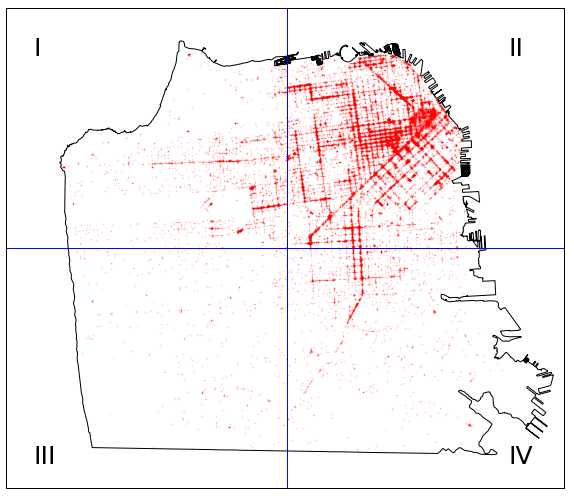
\includegraphics[width=\linewidth]{plots/grid1-cropped.png}
  \caption{We divide San Francisco into 4 equal-area nodes. Taxi trips from a typical weekday are plotted as red dots.}
  \label{fig:sf}
\end{figure}

\subsubsection{Demand for Mobility}

\subsubsection{Demand for Backup Power}
A key component of this analysis is to simulate the demand (and willingness to pay) for backup power due to power outages in each node. This work involves three key components: (1) representing outages in each node, (2) quantifying the magnitude of unserved load, (3) estimating price for supplying backup power. The present work focuses on task 1, making simplified assumptions based on the literature for tasks 2 and 3. 

To represent outages, we draw on historical outage data from Pacific Gas \& Electric Co. The data are collected using an automated web scraper that collects information about ongoing power outages every 8 minutes. The information include the locations of all ongoing outages and the number of customers affected at each location. We aggregate outages reported in each node to estimate the number of customers affected in each node at a given time.

In the present analysis, we examine two separate days of outage data, including both ``typical'' and ``extreme'' outage scenarios. We use outage data for September 29, 2014 to represent a typical day and December 31, 2014 to represent an extreme day. Figures \ref{fig:typical_day} and \ref{fig:extreme_day} show the number of customers without power in each node and across all nodes at each time step.

Currently, we assume electricity demand is constant at all time steps for all customers in a node. Demand in each node will consider the likely breakdown among residential, commercial and industrial customers, applying different rules of thumb regarding power demand for each customer type. Future iterations of the model can include time-varying demand profiles that better represent the magnitude of unserved loads. We assign a fixed cost per kWh discharge to the grid. Future work will examine a dynamic price per kWh affected by (1) the magnitude of unserved loads, and (2) outage duration.

\begin{figure}[!htbp]
  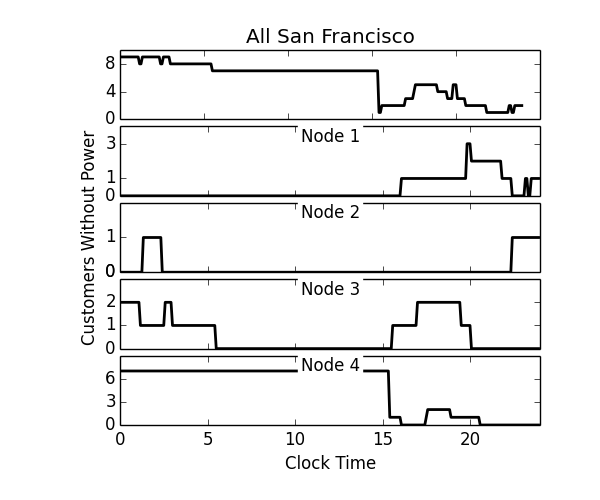
\includegraphics[width=\linewidth]{plots/typical_day_2014929.png}
  \caption{Number of customers without power overall (top) and in each node on September 29, 2014. The represented outage data will serve as our typical outage scenario.}
  \label{fig:typical_day}
\end{figure}

\begin{figure}[!htbp]
  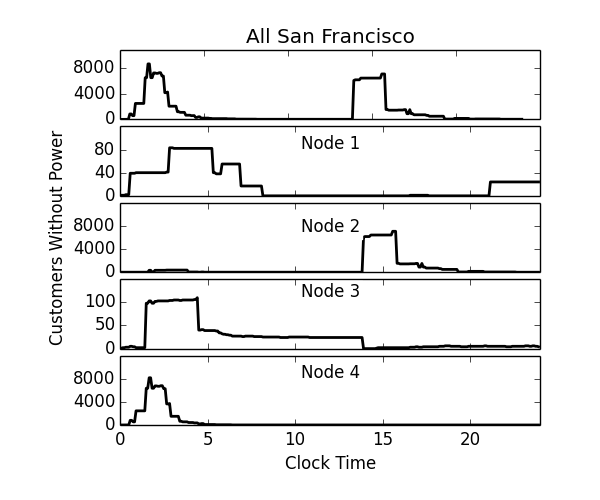
\includegraphics[width=\linewidth]{plots/extreme_day_20141231.png}
  \caption{Number of customers without power overall (top) and in each node on December 31, 2014. The represented outage data will serve as our extreme outage scenario.}
  \label{fig:extreme_day}
\end{figure}


\section{Discussion}

\section{Summary}


%%%% EXTRA STUFF WE MIGHT WANT LATER

%Later:

%\subsection{Discretization}

%\begin{eqnarray*}
    %u_{i,k}^{n+1} &=& u_{i,k}^{n} - \frac{q_C \Delta t}{2 \Delta x}\left(u_{i,k+1}^{n} - u_{i,k-1}^{n} \right) + \\
    %&& \frac{(q_C \Delta t)^2}{2 (\Delta x)^2}\left(u_{i,k+1}^{n} - 2u_{i,k}^{n} + u_{i,k-1}^{n} \right) + \sigma_{I_i \rightarrow C_i,k}^n \\
    %v_{i,k}^{n+1} &=& v_{i,k}^{n} + \Delta t \sum_{j\in\mathbb{Z}} \left[ \sigma_{I_i \leftarrow I_j,k}^{\prime,n} + \sigma_{I_i \leftarrow I_j,k}^{o,n} \right. \\
    %& & ~~~ \left. - \sigma_{I_i \rightarrow I_j,k}^{\prime,n} - \sigma_{I_i \rightarrow I_j,k}^{o,n} \right] \\
    %&& ~~~ - \Delta t \left( \sigma_{I_i \rightarrow C_i,k}^n + \sigma_{I_i \rightarrow D_i,k}^n \right) \\
    %w_{i,k}^{n+1} &=& w_{i,k}^{n} - \frac{q_D \Delta t}{2 \Delta x}\left(w_{i,k+1}^{n} - w_{i,k-1}^{n} \right) + \\
    %&& \frac{(q_D \Delta t)^2}{2 (\Delta x)^2}\left(w_{i,k+1}^{n} - 2w_{i,k}^{n} + w_{i,k-1}^{n} \right) + \sigma_{I_i \rightarrow D_i,k}^n \\   
%\end{eqnarray*}

%\begin{eqnarray*}
    %K &=& \sum_{i\in\mathbb{Z}} \int_{t=0}^{T} \left[ \rho_{disch}(Q_{dis,i}(t)) Q_{dis,i}(t) + \right. \\ && \left. \rho_{mob}\left(\sum_{j\in\mathbb{Z}}Q_{mob,i}(t)\right)\sum_{j\in\mathbb{Z}}Q_{mob,i,j}(t) - CQ_{ch,i}(t) \right]\\
%\end{eqnarray*}


%\begin{eqnarray*}
%q_C(x) &=& \frac{P(x)}{E_{max}}\eta(x)\frac{1}{60} \\
%P(x) &=& \begin{cases} 
      %50 & x/E_{max} < 0.8 \\
      %-860(x/E_{max}) + 738 & 0.8 \leq x/E_{max} < 0.85 \\
      %-55(x/E_{max}) + 53.75 & 0.85 \leq x/E_{max} < 0.95 \\
      %1.5 & 0.95 \leq x/E_{max}
   %\end{cases}  \\
  %\eta(x) &=& ??? \\
  %q_D(x) &=& \frac{-20}{E_{max}}\frac{1}{60}
%\end{eqnarray*}


%The charging rate defined by $P(x)$ is illustrated in Figure \ref{fig:dcFastRate}. The function is assumed to be piecewise linear and it rapidly transforms after an SOC of 80\% from a fast charge to a Level 2 charge (7kW) and then declines again to a trickle charge at an SOC of 95\%.
% plot(seq(0,1,by=.01),c(rep(50,80),-860*seq(.8,.84,by=.01)+738,-55*seq(.85,.94,by=.01)+53.75,rep(1.5,6)),type='l',xlab="SOC",ylab="Power (kW)",main="DC Fast Charging Rate")
% grid()
% points(seq(0,1,by=.01),c(rep(50,80),-860*seq(.8,.84,by=.01)+738,-55*seq(.85,.94,by=.01)+53.75,rep(1.5,6)),type='l')
%\begin{figure}[!htbp]
%\centering
%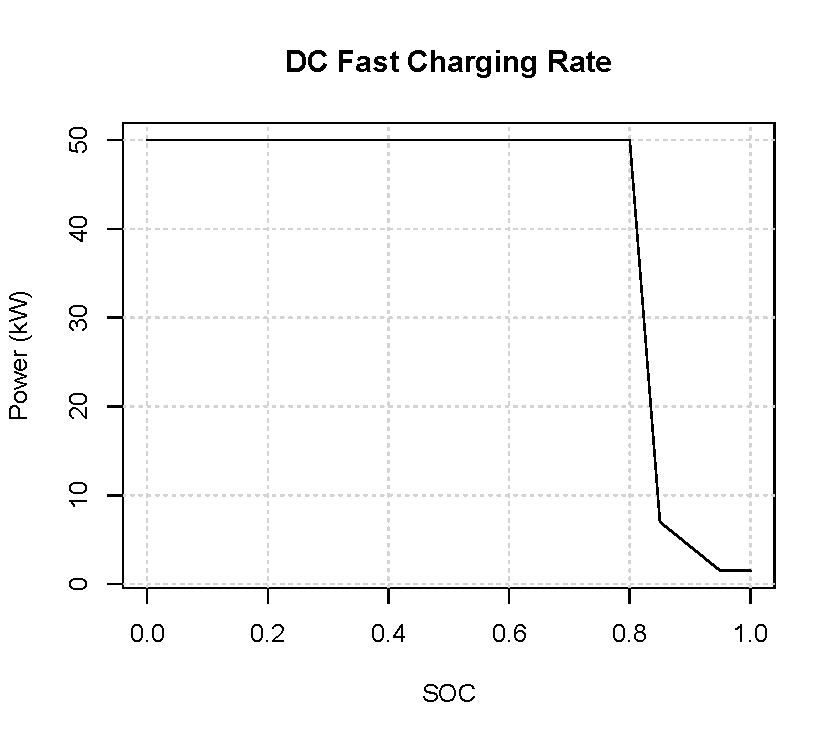
\includegraphics[width=3.0in]{dcFastRate} 
%\caption{The function $P(x)$, or the charge rate of a DC Fast charger.}
%\label{fig:dcFastRate}
%\end{figure}



% needed in second column of first page if using \IEEEpubid
%\IEEEpubidadjcol

% An example of a floating figure using the graphicx package.
% Note that \label must occur AFTER (or within) \caption.
% For figures, \caption should occur after the \includegraphics.
% Note that IEEEtran v1.7 and later has special internal code that
% is designed to preserve the operation of \label within \caption
% even when the captionsoff option is in effect. However, because
% of issues like this, it may be the safest practice to put all your
% \label just after \caption rather than within \caption{}.
%
% Reminder: the "draftcls" or "draftclsnofoot", not "draft", class
% option should be used if it is desired that the figures are to be
% displayed while in draft mode.
%
%\begin{figure}[!t]
%\centering
%\includegraphics[width=2.5in]{myfigure}
% where an .eps filename suffix will be assumed under latex, 
% and a .pdf suffix will be assumed for pdflatex; or what has been declared
% via \DeclareGraphicsExtensions.
%\caption{Simulation Results}
%\label{fig_sim}
%\end{figure}

% Note that IEEE typically puts floats only at the top, even when this
% results in a large percentage of a column being occupied by floats.


% An example of a double column floating figure using two subfigures.
% (The subfig.sty package must be loaded for this to work.)
% The subfigure \label commands are set within each subfloat command, the
% \label for the overall figure must come after \caption.
% \hfil must be used as a separator to get equal spacing.
% The subfigure.sty package works much the same way, except \subfigure is
% used instead of \subfloat.
%
%\begin{figure*}[!t]
%\centerline{\subfloat[Case I]\includegraphics[width=2.5in]{subfigcase1}%
%\label{fig_first_case}}
%\hfil
%\subfloat[Case II]{\includegraphics[width=2.5in]{subfigcase2}%
%\label{fig_second_case}}}
%\caption{Simulation results}
%\label{fig_sim}
%\end{figure*}
%
% Note that often IEEE papers with subfigures do not employ subfigure
% captions (using the optional argument to \subfloat), but instead will
% reference/describe all of them (a), (b), etc., within the main caption.


% An example of a floating table. Note that, for IEEE style tables, the 
% \caption command should come BEFORE the table. Table text will default to
% \footnotesize as IEEE normally uses this smaller font for tables.
% The \label must come after \caption as always.
%
%\begin{table}[!t]
%% increase table row spacing, adjust to taste
%\renewcommand{\arraystretch}{1.3}
% if using array.sty, it might be a good idea to tweak the value of
% \extrarowheight as needed to properly center the text within the cells
%\caption{An Example of a Table}
%\label{table_example}
%\centering
%% Some packages, such as MDW tools, offer better commands for making tables
%% than the plain LaTeX2e tabular which is used here.
%\begin{tabular}{|c||c|}
%\hline
%One & Two\\
%\hline
%Three & Four\\
%\hline
%\end{tabular}
%\end{table}


% Note that IEEE does not put floats in the very first column - or typically
% anywhere on the first page for that matter. Also, in-text middle ("here")
% positioning is not used. Most IEEE journals use top floats exclusively.
% Note that, LaTeX2e, unlike IEEE journals, places footnotes above bottom
% floats. This can be corrected via the \fnbelowfloat command of the
% stfloats package.



% \section{Conclusion}





% if have a single appendix:
%\appendix[Proof of the Zonklar Equations]
% or
%\appendix  % for no appendix heading
% do not use \section anymore after \appendix, only \section*
% is possibly needed

% use appendices with more than one appendix
% then use \section to start each appendix
% you must declare a \section before using any
% \subsection or using \label (\appendices by itself
% starts a section numbered zero.)
%


% \appendices
% \section{Proof of the First Zonklar Equation}
% Some text for the appendix.

% % use section* for acknowledgement
% \section*{Acknowledgment}


% The authors would like to thank...


% % Can use something like this to put references on a page
% % by themselves when using endfloat and the captionsoff option.
% \ifCLASSOPTIONcaptionsoff
%   \newpage
% \fi



% trigger a \newpage just before the given reference
% number - used to balance the columns on the last page
% adjust value as needed - may need to be readjusted if
% the document is modified later
%\IEEEtriggeratref{8}
% The "triggered" command can be changed if desired:
%\IEEEtriggercmd{\enlargethispage{-5in}}

% references section

% can use a bibliography generated by BibTeX as a .bbl file
% BibTeX documentation can be easily obtained at:
% http://www.ctan.org/tex-archive/biblio/bibtex/contrib/doc/
% The IEEEtran BibTeX style support page is at:
% http://www.michaelshell.org/tex/ieeetran/bibtex/
\bibliographystyle{IEEEtran}
% argument is your BibTeX string definitions and bibliography database(s)
\bibliography{refs} 
%
% <OR> manually copy in the resultant .bbl file
% set second argument of \begin to the number of references
% (used to reserve space for the reference number labels box)
%\begin{thebibliography}{1}

% \bibitem{IEEEhowto:kopka}
% H.~Kopka and P.~W. Daly, \emph{A Guide to \LaTeX}, 3rd~ed.\hskip 1em plus
%   0.5em minus 0.4em\relax Harlow, England: Addison-Wesley, 1999.

%\end{thebibliography}

% biography section
% 
% If you have an EPS/PDF photo (graphicx package needed) extra braces are
% needed around the contents of the optional argument to biography to prevent
% the LaTeX parser from getting confused when it sees the complicated
% \includegraphics command within an optional argument. (You could create
% your own custom macro containing the \includegraphics command to make things
% simpler here.)
%\begin{biography}[{\includegraphics[width=1in,height=1.25in,clip,keepaspectratio]{mshell}}]{Michael Shell}
% or if you just want to reserve a space for a photo:

% \begin{IEEEbiography}[{\includegraphics[width=1in,height=1.25in,clip,keepaspectratio]{picture}}]{John Doe}
% \blindtext
% \end{IEEEbiography}

% You can push biographies down or up by placing
% a \vfill before or after them. The appropriate
% use of \vfill depends on what kind of text is
% on the last page and whether or not the columns
% are being equalized.

%\vfill

% Can be used to pull up biographies so that the bottom of the last one
% is flush with the other column.
%\enlargethispage{-5in}



% that's all folks
\end{document}

